\section{推前测度的构造}
\label{sec:push-construction}

可测映射保证目标空间中的集合问题在原空间有意义：目标可测集的原像仍然可测。若原空间还配有测度，就可以回答“映射的输出落在$B$中的质量有多少”：把会被送进$B$的点全部找出来，累计它们的质量。本节用这一想法定义推前测度，核对它的可数可加性与复合规则，再用例子观察不同映射怎样改变质量的分配。积分与密度的计算放在后两节。

\subsection{推前测度的定义}
\label{sec:push-definition}

设$(X,\mathcal A)$与$(Y,\mathcal B)$是可测空间，$T:X\to Y$可测，$\mu$是$(X,\mathcal A)$上的测度。对$B\in\mathcal B$，输出落在$B$中的点恰好组成原像$T^{-1}(B)=\{x\in X:T(x)\in B\}$，它属于$\mathcal A$，于是可以取它的质量作为$B$的质量。

\begin{definition}[推前测度]
\label{def:push-pushforward}
在上述记号下，令
\[
(T_\#\mu)(B)=\mu\bigl(T^{-1}(B)\bigr),\qquad B\in\mathcal B ,
\]
称$T_\#\mu$为$\mu$在$T$下的\term{推前测度}（pushforward measure）。
\end{definition}

定义只用原像，所以先要核对$T_\#\mu$确实是测度。空集的原像是空集，故$(T_\#\mu)(\varnothing)=0$。设$B_1,B_2,\ldots\in\mathcal B$两两不交，则它们的原像也两两不交：一个$x$若同时属于$T^{-1}(B_n)$与$T^{-1}(B_m)$，$T(x)$就同时属于$B_n$与$B_m$。原像保持并运算，$T^{-1}(\bigcup_nB_n)=\bigcup_nT^{-1}(B_n)$，由$\mu$的可数可加性，
\[
(T_\#\mu)\Bigl(\bigcup_nB_n\Bigr)=\mu\Bigl(\bigcup_nT^{-1}(B_n)\Bigr)=\sum_n\mu\bigl(T^{-1}(B_n)\bigr)=\sum_n(T_\#\mu)(B_n).
\]
所以$T_\#\mu$是$(Y,\mathcal B)$上的测度。又$T^{-1}(Y)=X$，总质量不变：$(T_\#\mu)(Y)=\mu(X)$。特别地，有限测度推前后仍有限，概率测度推前后仍是概率测度。

\paragraph{复合规则}
复杂的映射常常可以拆成几步简单的映射。设$S:(Y,\mathcal B)\to(Z,\mathcal C)$也可测，复合$S\circ T$可测，并且原像按逆序作用：$(S\circ T)^{-1}(C)=T^{-1}(S^{-1}(C))$。于是对$C\in\mathcal C$，
\[
\bigl((S\circ T)_\#\mu\bigr)(C)=\mu\bigl(T^{-1}(S^{-1}(C))\bigr)=(T_\#\mu)\bigl(S^{-1}(C)\bigr)=\bigl(S_\#(T_\#\mu)\bigr)(C),
\]
即$(S\circ T)_\#\mu=S_\#(T_\#\mu)$。分两步传递质量与一步传递质量的结果相同，所以可以把映射拆开逐步计算推前。

\paragraph{总质量保持，$\sigma$有限性未必保持}
总质量不变，但$\sigma$有限性可能丢失，因为推前可以把无限多份有限质量集中到一点。在$\mathbb N$上取计数测度$\mu$，它是$\sigma$有限的。令$T$把$\mathbb N$映到单点集$Y=\{y\}$，则$(T_\#\mu)(\{y\})=\mu(\mathbb N)=+\infty$；$Y$的可测子集只有$\varnothing$与$\{y\}$，无法写成有限质量集合的可数并。后面需要测度延拓的唯一性或Radon–Nikodym定理时，推前测度的$\sigma$有限性必须单独核对。

\subsection{映射下的质量转移}
\label{sec:push-mass-transfer}

定义只说明了怎样计算，下面用例子看推前测度到底记录了什么。我们先按原像确定目标测度，不预设它有任何密度。

\paragraph{一一映射与多对一映射}
若$T$是一一映射，每个输出点只收到一个原像的质量，推前只是把质量换了位置。设$X=\{1,2,3,4\}$上的测度$\mu$给四个点分别赋权$0.1,0.2,0.3,0.4$，$T$把$k$送到$Y=\{a,b,c,d\}$中的第$k$个点，则$T_\#\mu$给$a,b,c,d$的权重仍是$0.1,0.2,0.3,0.4$。

推前不要求$T$是单射。若几个点被送到同一个输出，它们的质量在输出处相加。仍取上面的$\mu$，令$T(1)=T(3)=a$，$T(2)=T(4)=b$，则$T^{-1}(\{a\})=\{1,3\}$，$T^{-1}(\{b\})=\{2,4\}$，所以
\[
T_\#\mu=0.4\,\delta_a+0.6\,\delta_b .
\]
原来的四个点在输出端只剩两个，总量仍为$1$，见图~\ref{fig:push-merge}(a)。从$T_\#\mu$出发已经无法分辨$a$处的$0.4$来自哪两个点，汇合丢掉了原像之间的区分。

推前还可以把连续分布的质量汇合成点质量。令$\mu=\lambda|_{[0,1]}$，$T(x)=\lfloor2x\rfloor$。$[0,1]$中的原像分别是$T^{-1}(\{0\})\cap[0,1]=[0,\tfrac12)$，$T^{-1}(\{1\})\cap[0,1]=[\tfrac12,1)$，$T^{-1}(\{2\})\cap[0,1]=\{1\}$，所以$T_\#\mu=\tfrac12\delta_0+\tfrac12\delta_1$。每个单点在$\mu$下质量为零，推前后却出现了质量$\tfrac12$的点，因为原像不是单点，而是一段区间。

\begin{figure}[!htbp]
  \centering
  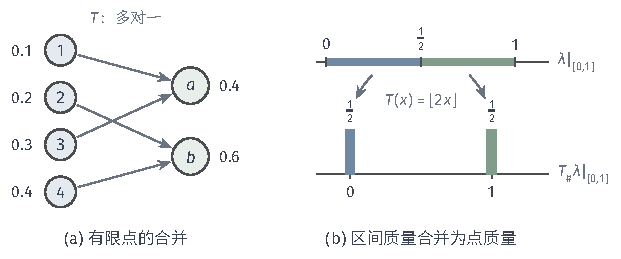
\includegraphics[width=105.1mm]{figures/02-abstract-mathematics/01-metric-and-measure/tikz/c2-pushforward-merge/figure.pdf}
  \caption{推前测度累计原像的质量。(a)四个带权点经多对一映射送到$a,b$两点，$a$收集点$1,3$的权重$0.1+0.3=0.4$，$b$收集点$2,4$的权重$0.2+0.4=0.6$；(b)$[0,1]$上的长度测度经$T(x)=\lfloor2x\rfloor$推前，原像$[0,\tfrac12)$与$[\tfrac12,1)$的长度分别汇集为点$0$和点$1$处的质量$\tfrac12$，单点$\{1\}$的长度为零，不贡献质量。}
  \label{fig:push-merge}
\end{figure}

\paragraph{平移与伸缩}
在实轴上，平移$T(x)=x+t$满足$T^{-1}(B)=B-t$，由Lebesgue测度的平移不变性，$T_\#\lambda=\lambda$；这种使$T_\#\mu=\mu$的映射称为\term{保持测度}（measure-preserving）的映射。伸缩则改变长度。令$T(x)=2x$，区间$(a,b]$的原像是$(a/2,b/2]$，所以$(T_\#\lambda)((a,b])=(b-a)/2$。两个测度$T_\#\lambda$与$\tfrac12\lambda$在全部半开区间上一致，并在每个$(-n,n]$上有限，由测度延拓的唯一性，$T_\#\lambda=\tfrac12\lambda$。把实轴拉长一倍，同一个输出区间只收集到原来一半长度的输入。这个例子将在第~\ref{sec:push-smooth-change}小节用来核对坐标换元中因子的方向。

\paragraph{坐标投影}
多元问题中最常见的多对一映射是坐标投影。设$\mu$是$\mathcal B(\mathbb R^d)$上的测度，$1\leq k<d$，$\pi(\bm x)=(x_1,\ldots,x_k)$。$\pi$连续，因而Borel可测，且对$B\in\mathcal B(\mathbb R^k)$有$\pi^{-1}(B)=B\times\mathbb R^{d-k}$，所以
\[
(\pi_\#\mu)(B)=\mu\bigl(B\times\mathbb R^{d-k}\bigr).
\]
$\pi_\#\mu$称为$\mu$在前$k$个坐标上的\term{边缘测度}（marginal measure）。它只回答形如“前$k$个坐标落在$B$中”的问题，保留的是$\mu$在柱形集合$B\times\mathbb R^{d-k}$上的值；后$d-k$个坐标怎样分布、两组坐标之间怎样关联，都不再能从边缘测度读出。概率论中由联合分布得到边缘分布正是这一操作，可参考\BookChapterRef{chap:random-vectors}{卷七“随机向量与联合分布”章}。

\begin{example}[点质量与单位正方形的投影]
\label{ex:push-projection}
在$\mathbb R^2$上取$\mu=0.2\,\delta_{(0,0)}+0.3\,\delta_{(0,1)}+0.5\,\delta_{(1,1)}$。第一坐标的投影$\pi_1$把$(0,0)$与$(0,1)$都送到$0$，所以$(\pi_1)_\#\mu=0.5\,\delta_0+0.5\,\delta_1$；第二坐标的投影把$(0,1)$与$(1,1)$都送到$1$，所以$(\pi_2)_\#\mu=0.2\,\delta_0+0.8\,\delta_1$。两个边缘测度合起来也不能恢复$\mu$：四个格点上的质量只要横向与纵向的合计相同，边缘就相同。例如$0.1\,\delta_{(0,0)}+0.1\,\delta_{(1,0)}+0.4\,\delta_{(0,1)}+0.4\,\delta_{(1,1)}$的两个边缘也是$0.5\,\delta_0+0.5\,\delta_1$与$0.2\,\delta_0+0.8\,\delta_1$，它却给$(1,0)$正质量。

再取$\nu=\lambda_2|_{[0,1]^2}$。对$B=(a,b]$，$\pi_1^{-1}(B)\cap[0,1]^2=((a,b]\cap[0,1])\times[0,1]$是一个矩形，面积等于$\lambda((a,b]\cap[0,1])$。于是$(\pi_1)_\#\nu$与$\lambda|_{[0,1]}$在全部半开区间上一致，总量都为$1$，由延拓的唯一性，二者相等。图~\ref{fig:push-projection}画出了两种情形。
\end{example}

\begin{figure}[!htbp]
  \centering
  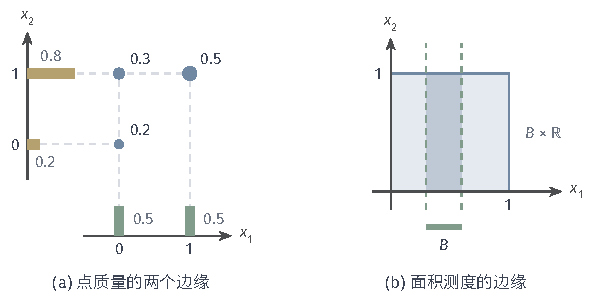
\includegraphics[width=100.9mm]{figures/02-abstract-mathematics/01-metric-and-measure/tikz/c2-projection-marginal/figure.pdf}
  \caption{坐标投影产生的边缘测度。(a)平面上三个点质量$0.2,0.3,0.5$，向横轴投影得到$0.5\delta_0+0.5\delta_1$，向纵轴投影得到$0.2\delta_0+0.8\delta_1$；(b)单位正方形上的面积测度，横轴区间$B$的边缘质量等于竖条$B\times\mathbb R$与正方形之交的面积，结果是$[0,1]$上的长度。}
  \label{fig:push-projection}
\end{figure}

边缘测度的总量与原测度相同，但$\sigma$有限性同样可能丢失：对整个平面上的$\lambda_2$，任一非退化区间$B$都有$(\pi_1)_\#\lambda_2(B)=\lambda_2(B\times\mathbb R)=+\infty$。上面的点质量例子还说明，输出测度不一定有密度，它可以是离散的。推前测度上的积分怎样计算，是下一节的问题；边缘测度何时有密度、怎样由原测度的密度算出，在第~\ref{sec:push-projection-density}小节处理。
